\section{Pendahuluan}
\subsection{Latar Belakang}
Fourier Transform digunakan untuk mengubah sinyal dari domain waktu (time domain) ke domain frekuensi (frequency domain). 
Dengan menggunakan Fourier Transform, sinyal dapat dianalisis dan dipahami lebih baik dalam hal komponen frekuensinya, amplitudonya, dan fase-nya. 
Fourier Transform sangat penting dalam berbagai aplikasi, seperti pengolahan sinyal audio, pengukuran, dan sistem monitoring.
\\\\
Ada dua jenis utama Fourier Transform: Transformasi Fourier Kontinu (Continuous Fourier Transform) dan Transformasi Fourier Diskrit (Discrete Fourier Transform). 
Transformasi Fourier Kontinu digunakan untuk sinyal kontinu dan didefinisikan dengan integral Fourier. 
Sementara itu, Transformasi Fourier Diskrit digunakan untuk sinyal diskrit dan didefinisikan dengan rumus yang lebih sederhana. 
Dalam prakteknya, Transformasi Fourier Diskrit lebih umum digunakan karena sinyal digital yang digunakan dalam komputer dan sistem lainnya adalah sinyal diskrit.

\subsection{Maksud dan Tujuan}
Memahami dasar-dasar teori Fourier Transform, termasuk perbedaan antara Transformasi Fourier Kontinu dan Diskrit.

\subsection{Hasil yang diharapkan}
Mengetahui perbandingan hasil sinyal Fourier Transform sebelum dan sesudah.

%===========================================================%
\section{Tugas Pendahuluan}
\begin{center}
	\colorbox{cyan!30}{\parbox{0.8\linewidth}{
    \begin{enumerate}
        \item Apa solusi lain ketika IPv4 habis, selain menggunakan IPv6?
        \item Sebutkan tiga keunggulan IPv6 dibandingkan IPv4!
        \item Mengapa panjang awal alamat IPv6 biasanya adalah 128 bit?
    \end{enumerate}}}
\end{center}

%===========================================================%
\section{Alat dan Bahan}
\begin{itemize}[label=$\bullet$, itemsep=-1pt, leftmargin=*]
	\item 1 Perangkat Arduino
	\item 1 Laptop
	\item 1 Osiloskop
	\item 1 Function Generator
	\item Software Arduino IDE
\end{itemize}

%===========================================================%
\section{Jangka Waktu Pelaksanaan}
Pemahaman dan konfigurasi 1 jam.

%===========================================================%
\section{Penjelasan dan Tahapan Konfigurasi}

%======================PERCOBAAN 1==========================%
\subsection{Percobaan 1}
\begin{center}

	\textbf{Memulai Arduino IDE}
	\begin{enumerate}
		\item Hubungkan Arduino Uno dengan laptop.
		\begin{figure}[H]
			\centering
			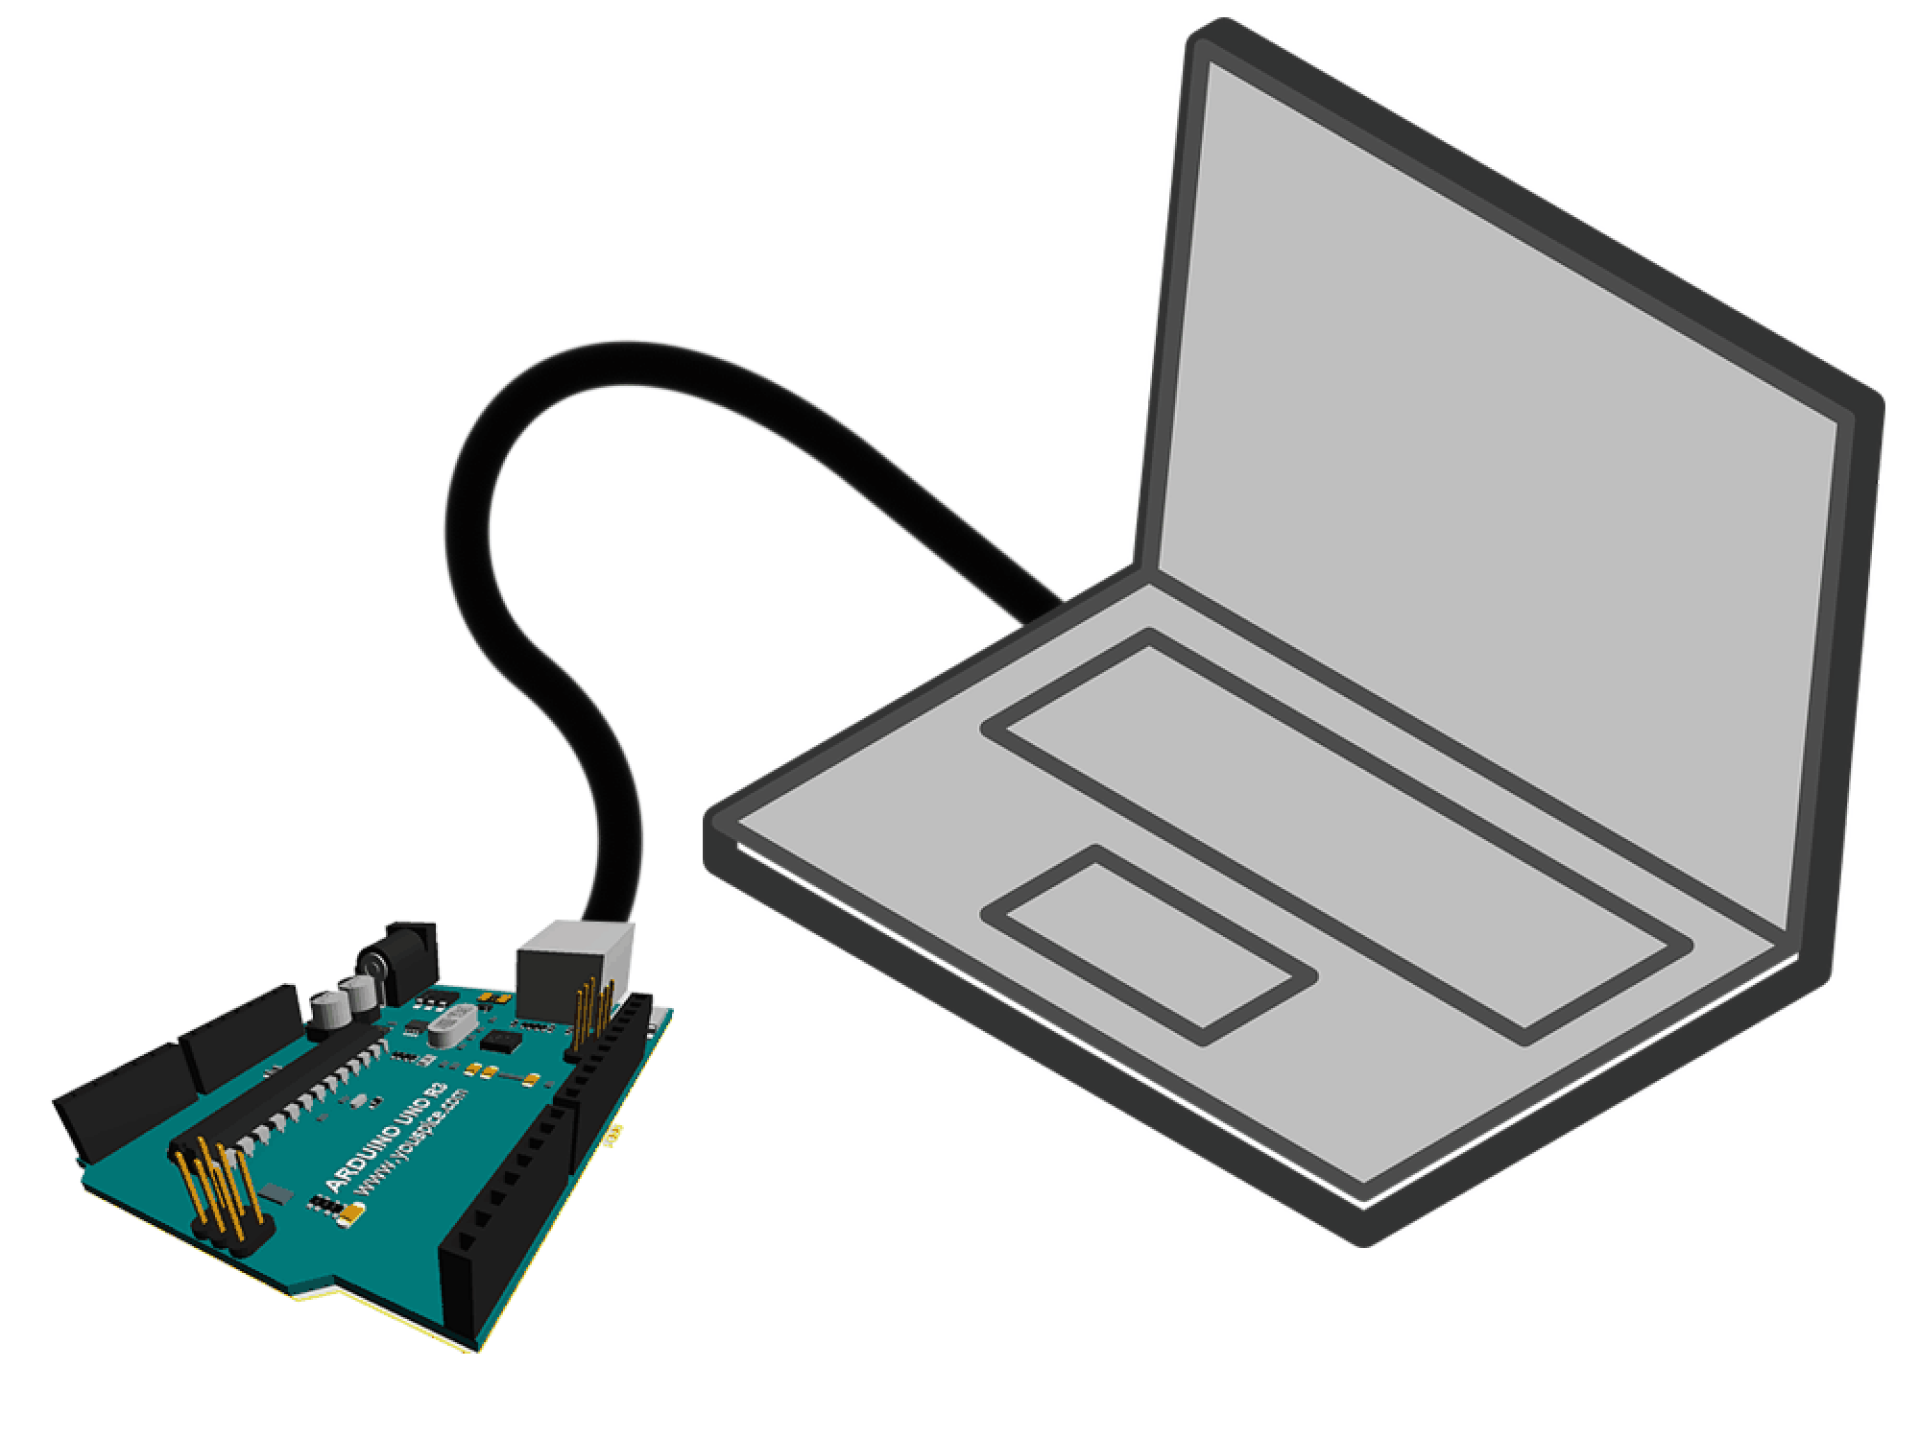
\includegraphics[width=0.8\linewidth]{P5/img/per1/step 1.png}
			\caption{Step 1}
			\label{fig:Step 1(Step 1)}
		\end{figure}
		\item Buka software Arduino IDE, lalu pilih new sketch.
		\begin{figure}[H]
			\centering
			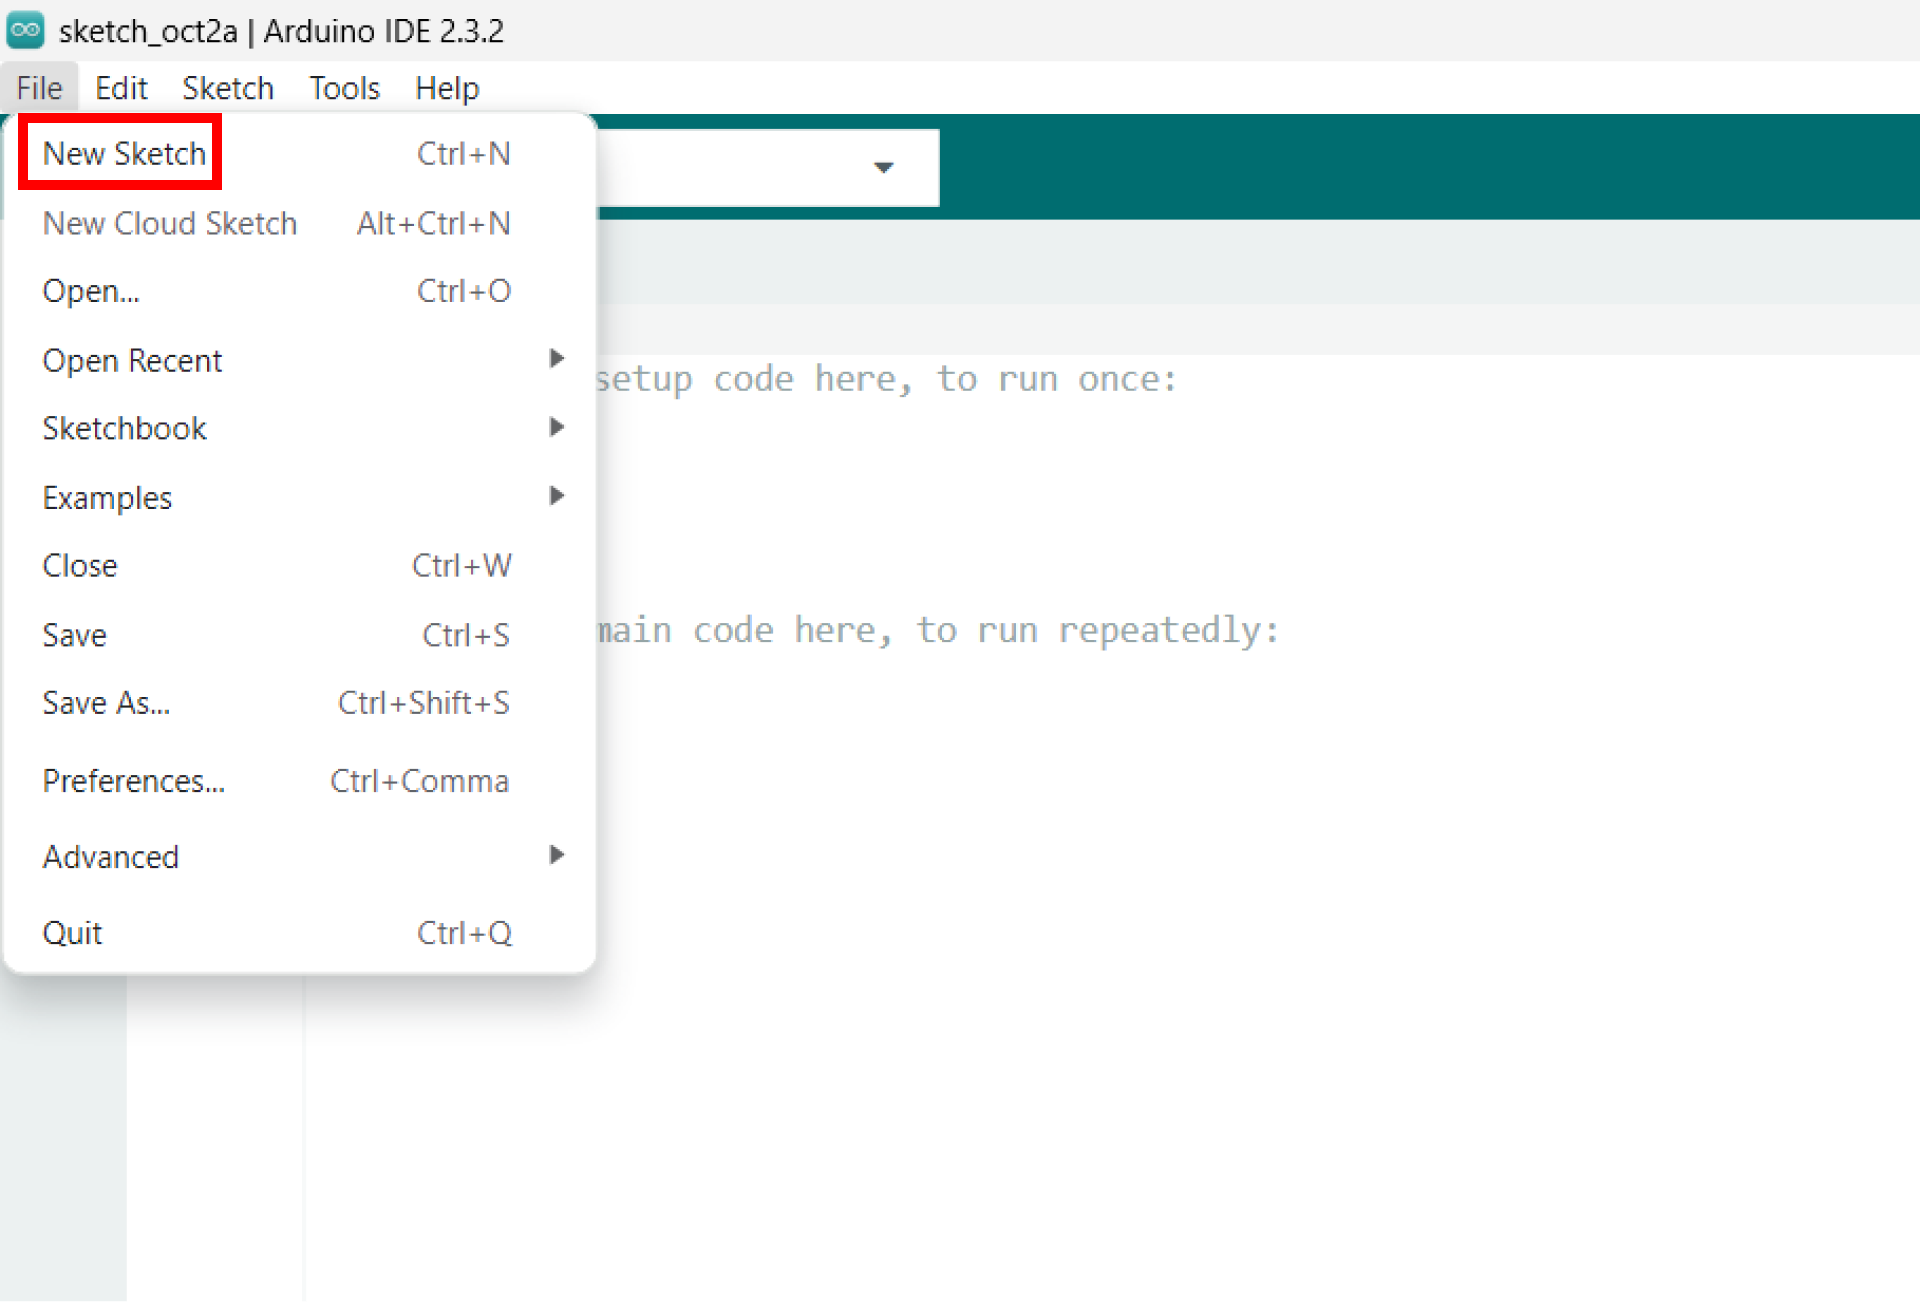
\includegraphics[width=0.8\linewidth]{P5/img/per1/step 2.png}
			\caption{Step 2}
			\label{fig:Step 2(Step 2)}
		\end{figure}
		\item Buka menu Tools, lalu cek Board dan Port yang terhubung apakah sudah benar
		\\(Port bergantung pada device, jadi bisa berbeda dengan port di Modul).
		\begin{figure}[H]
			\centering
			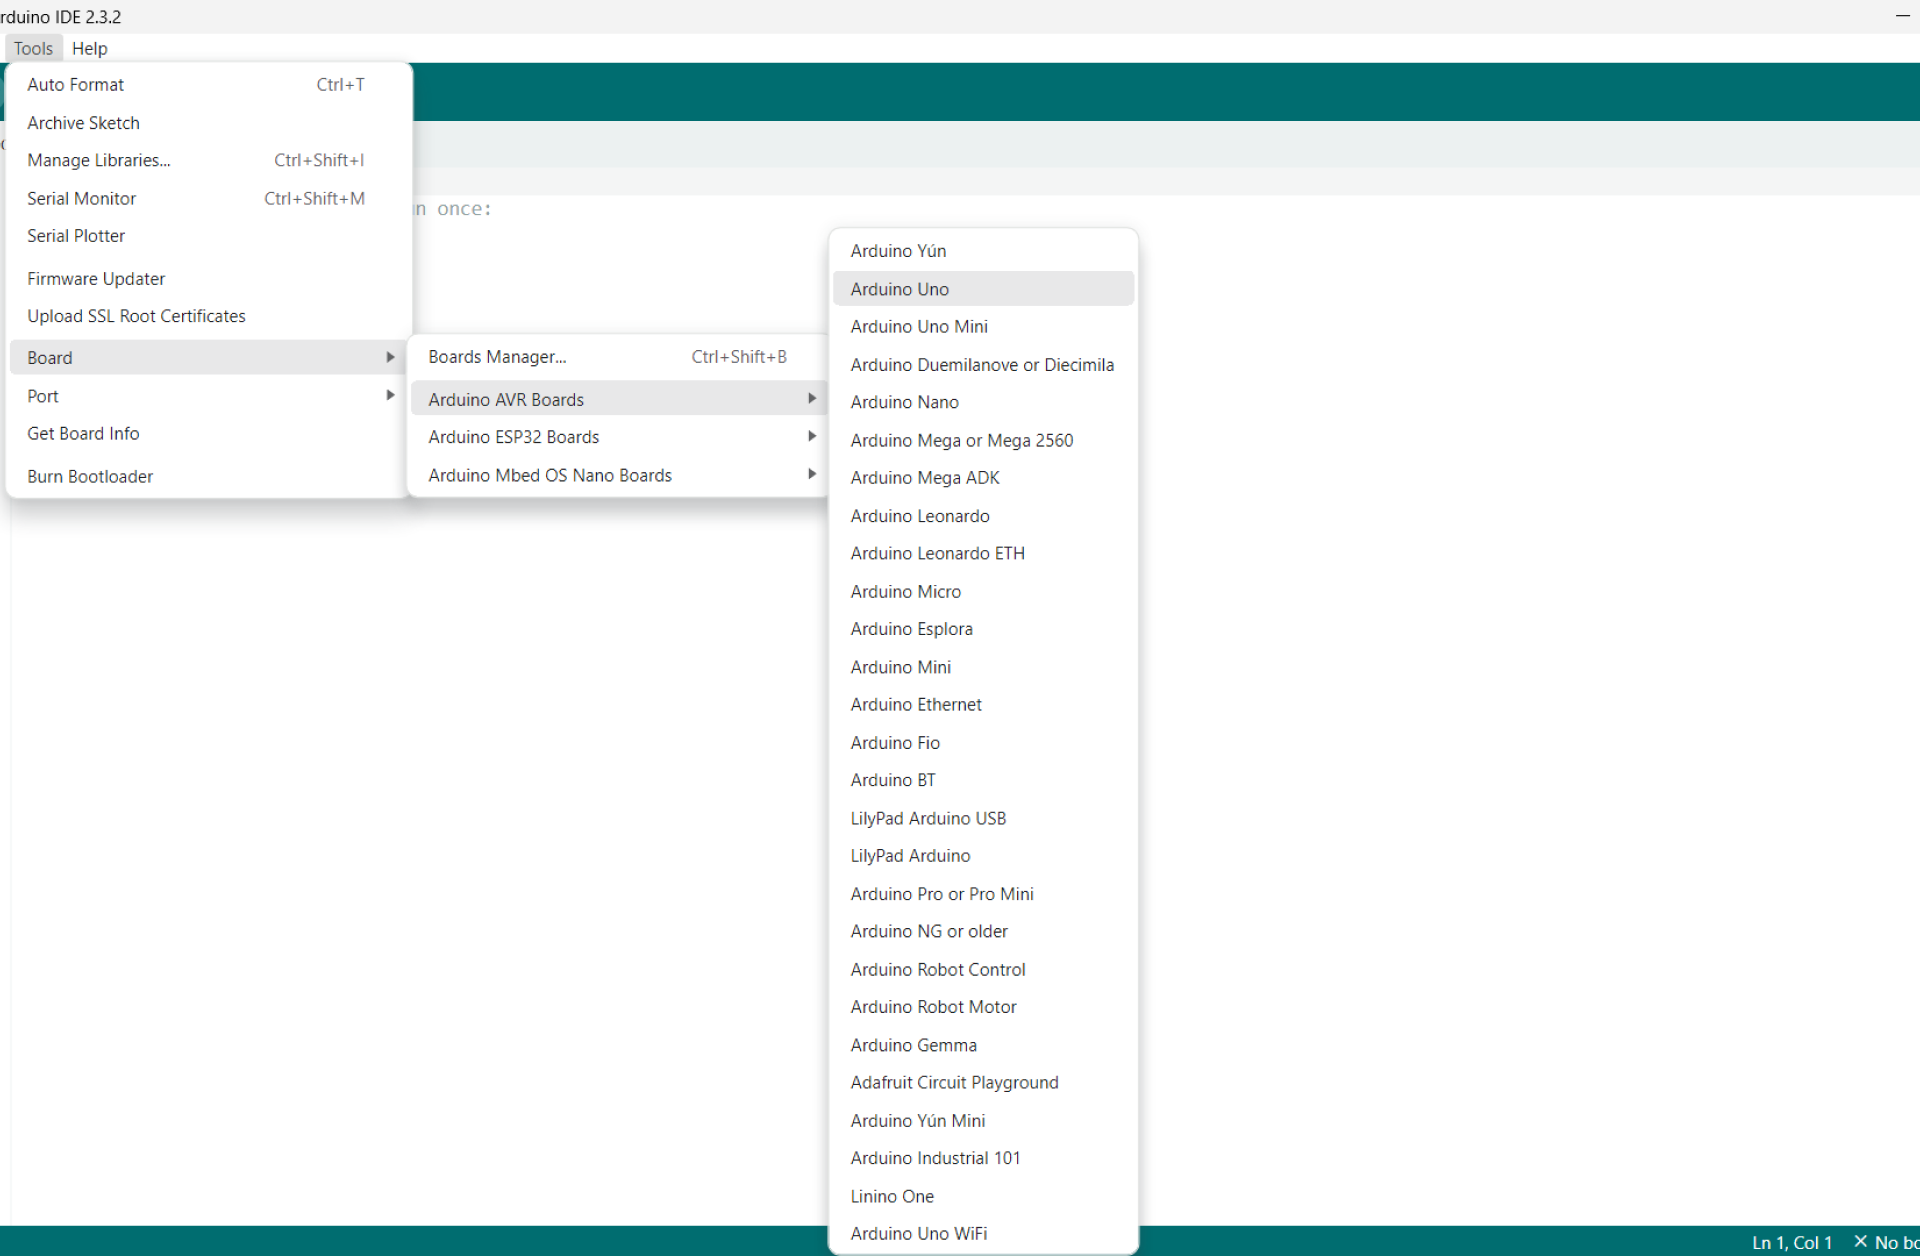
\includegraphics[width=0.8\linewidth]{P5/img/per1/step 3.png}
			\caption{Step 3}
			\label{fig:Step 3(Step 3)}
		\end{figure}
		\begin{figure}[H]
			\centering
			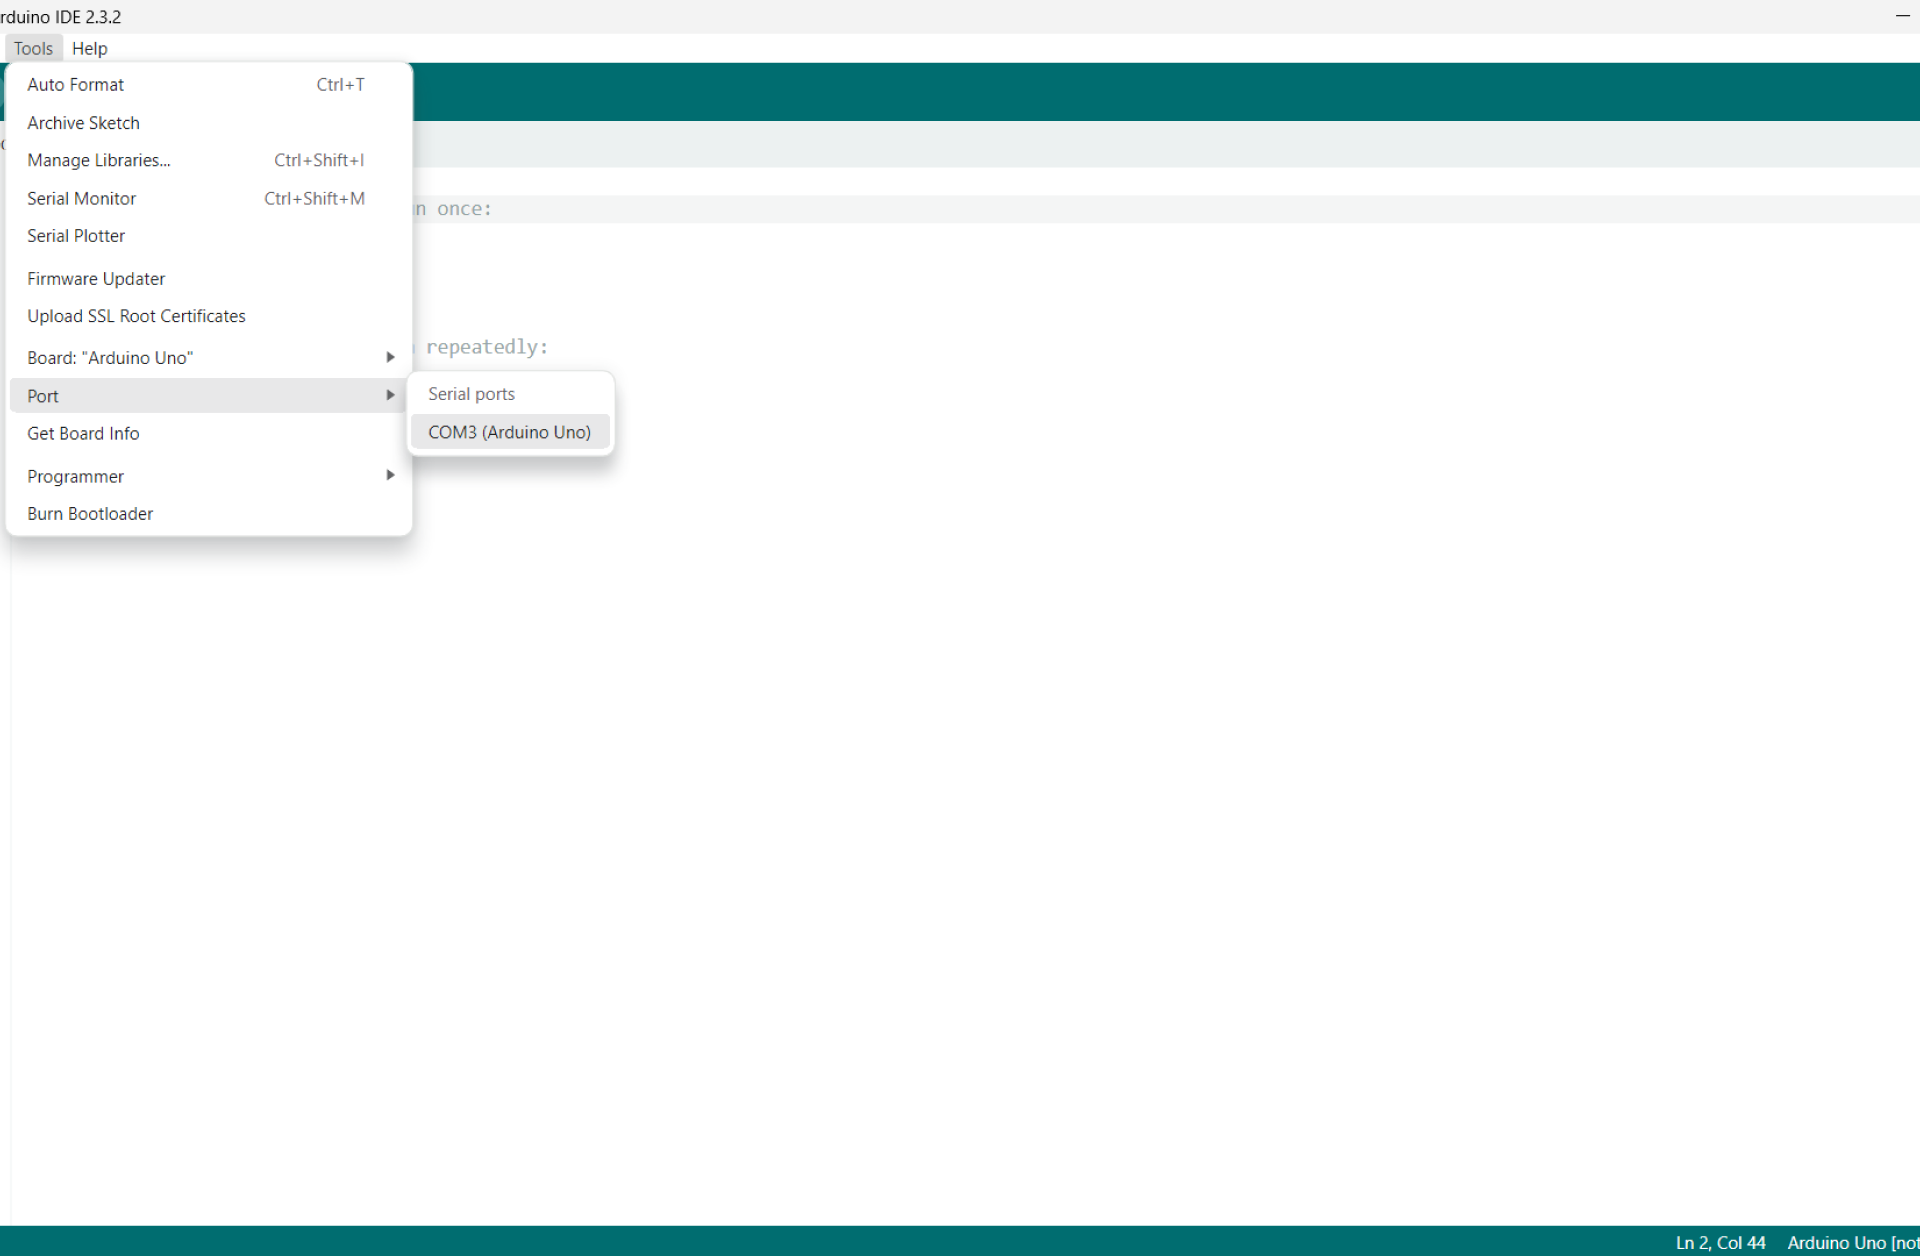
\includegraphics[width=0.8\linewidth]{P2/img/per1/step 4.png}
			\caption{Step 4}
			\label{fig:Step 4(Step 4)}
		\end{figure}

	
	\textbf{Kode Program Arduino}
		\item Masukkan kode program dibawah ini untuk menjalankan Fourier Transform pada Arduino IDE.
		\begin{figure}[H]
			\centering
			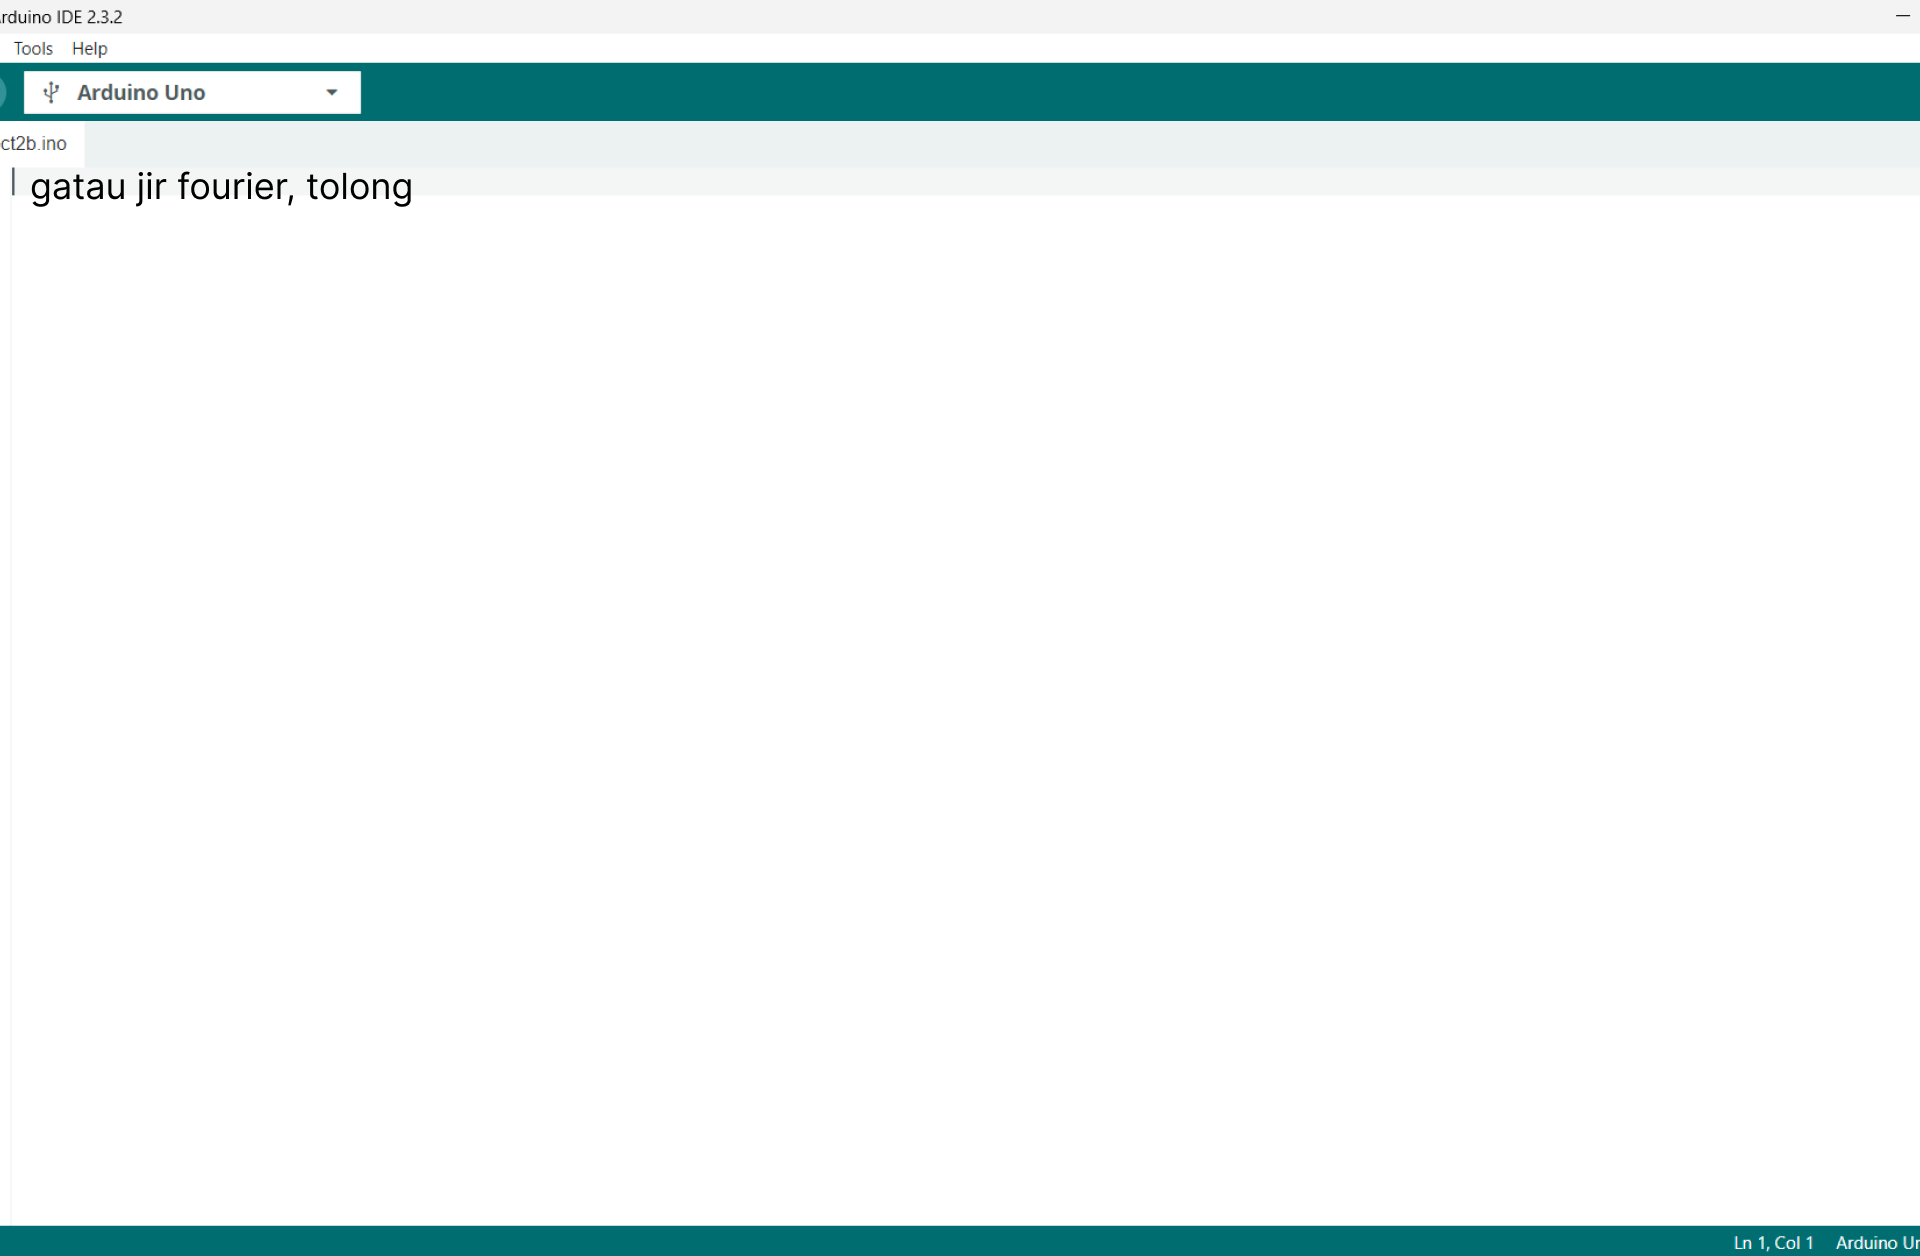
\includegraphics[width=0.8\linewidth]{P5/img/per1/step 5.png}
			\caption{Step 5}
			\label{fig:Step 5(Step 5)}
		\end{figure}
	
		\item Klik verify, apabila berhasil maka klik upload.
	\end{enumerate}
	
	\textbf{Memulai Function Generator}
	\begin{enumerate}
		\item Klik tombol power, untuk menyalakan function generator.
		\begin{figure}[H]
			\centering
			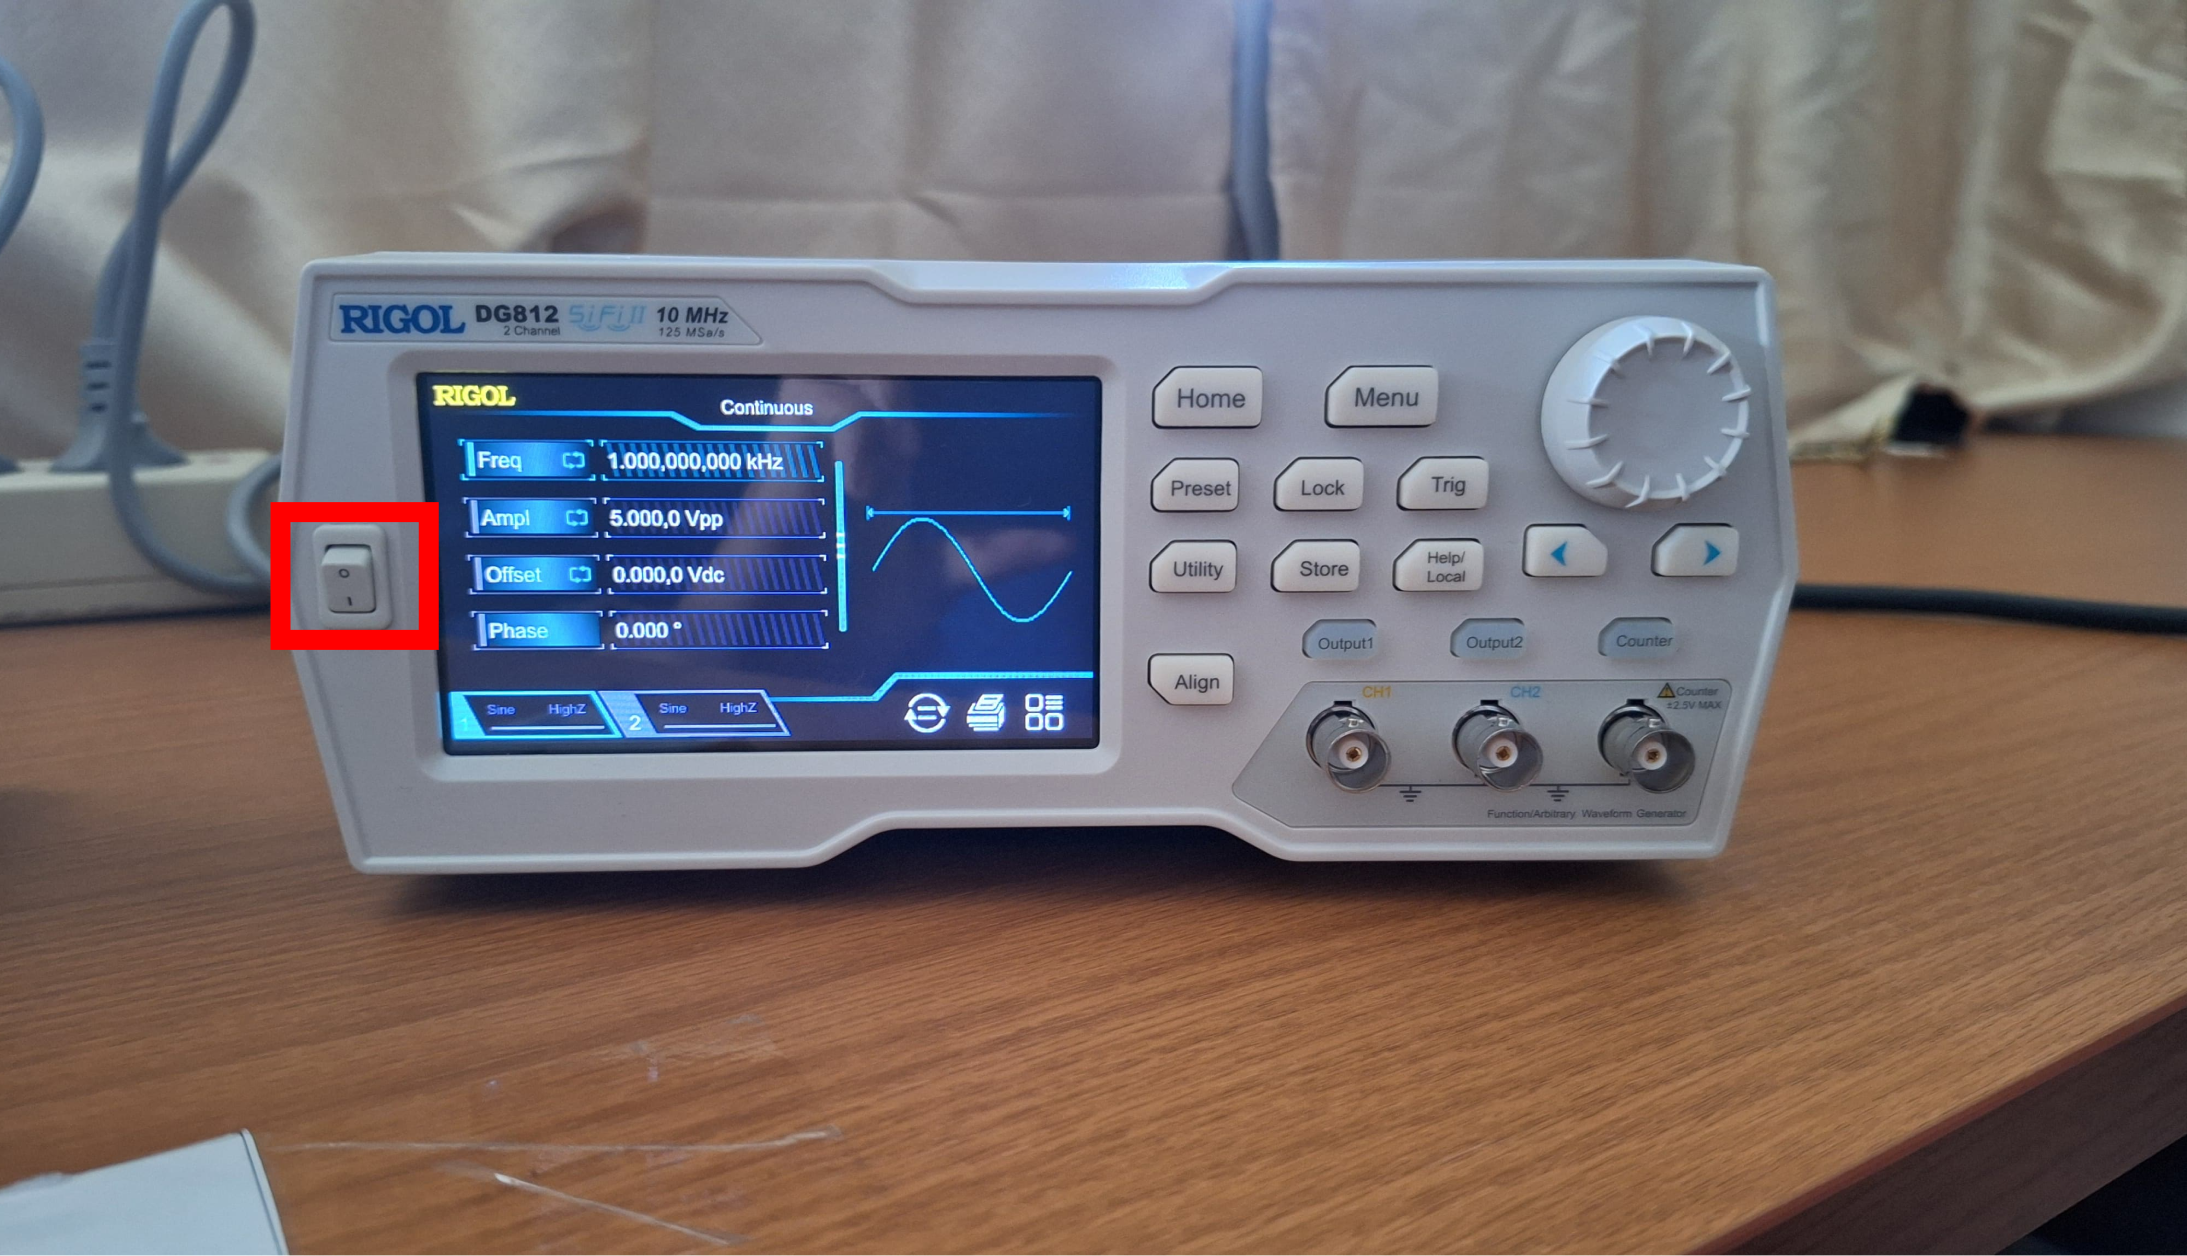
\includegraphics[width=0.8\linewidth]{P5/img/per1/step 6.png}
			\caption{Step 6}
			\label{fig:Step 6(Step 6)}
		\end{figure}

		\item Konfigurasi sinyal input pada Function generator.
		\begin{figure}[H]
			\centering
			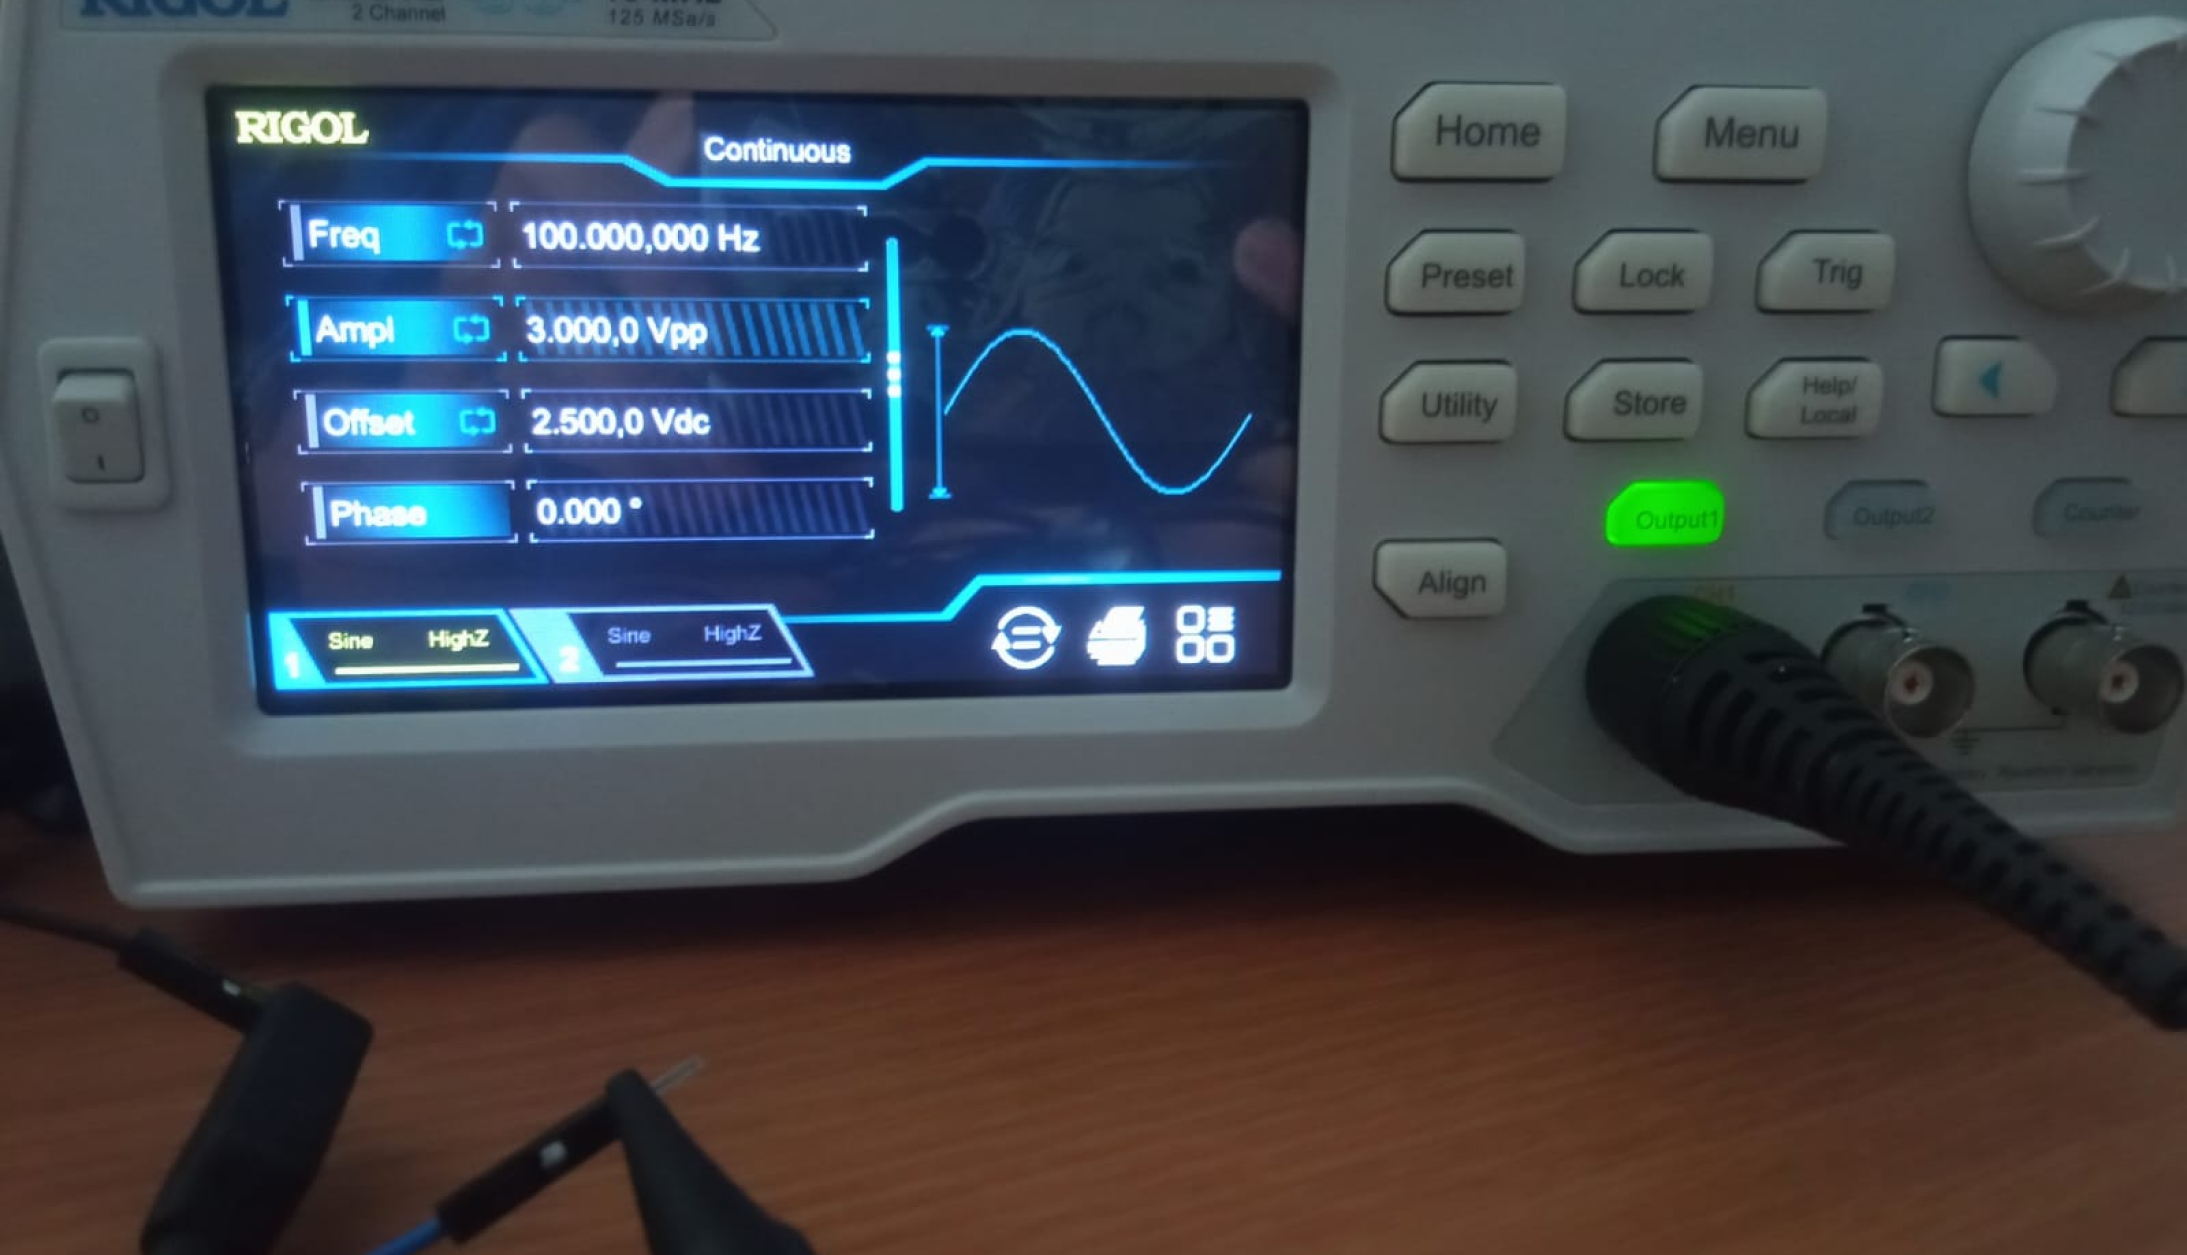
\includegraphics[width=0.8\linewidth]{P5/img/per1/step 7.png}
			\caption{Step 7}
			\label{fig:Step 7(Step 7)}
		\end{figure}
	\end{enumerate}

	\textbf{Konfigurasi Arduino}
	\begin{enumerate}
		\item Hubungkan kabel jumper ke salah satu pin Analog Arduino, kemudian hubungan ke probe.
		\\pengait (positif) Function generator.
		\begin{figure}[H]
			\centering
			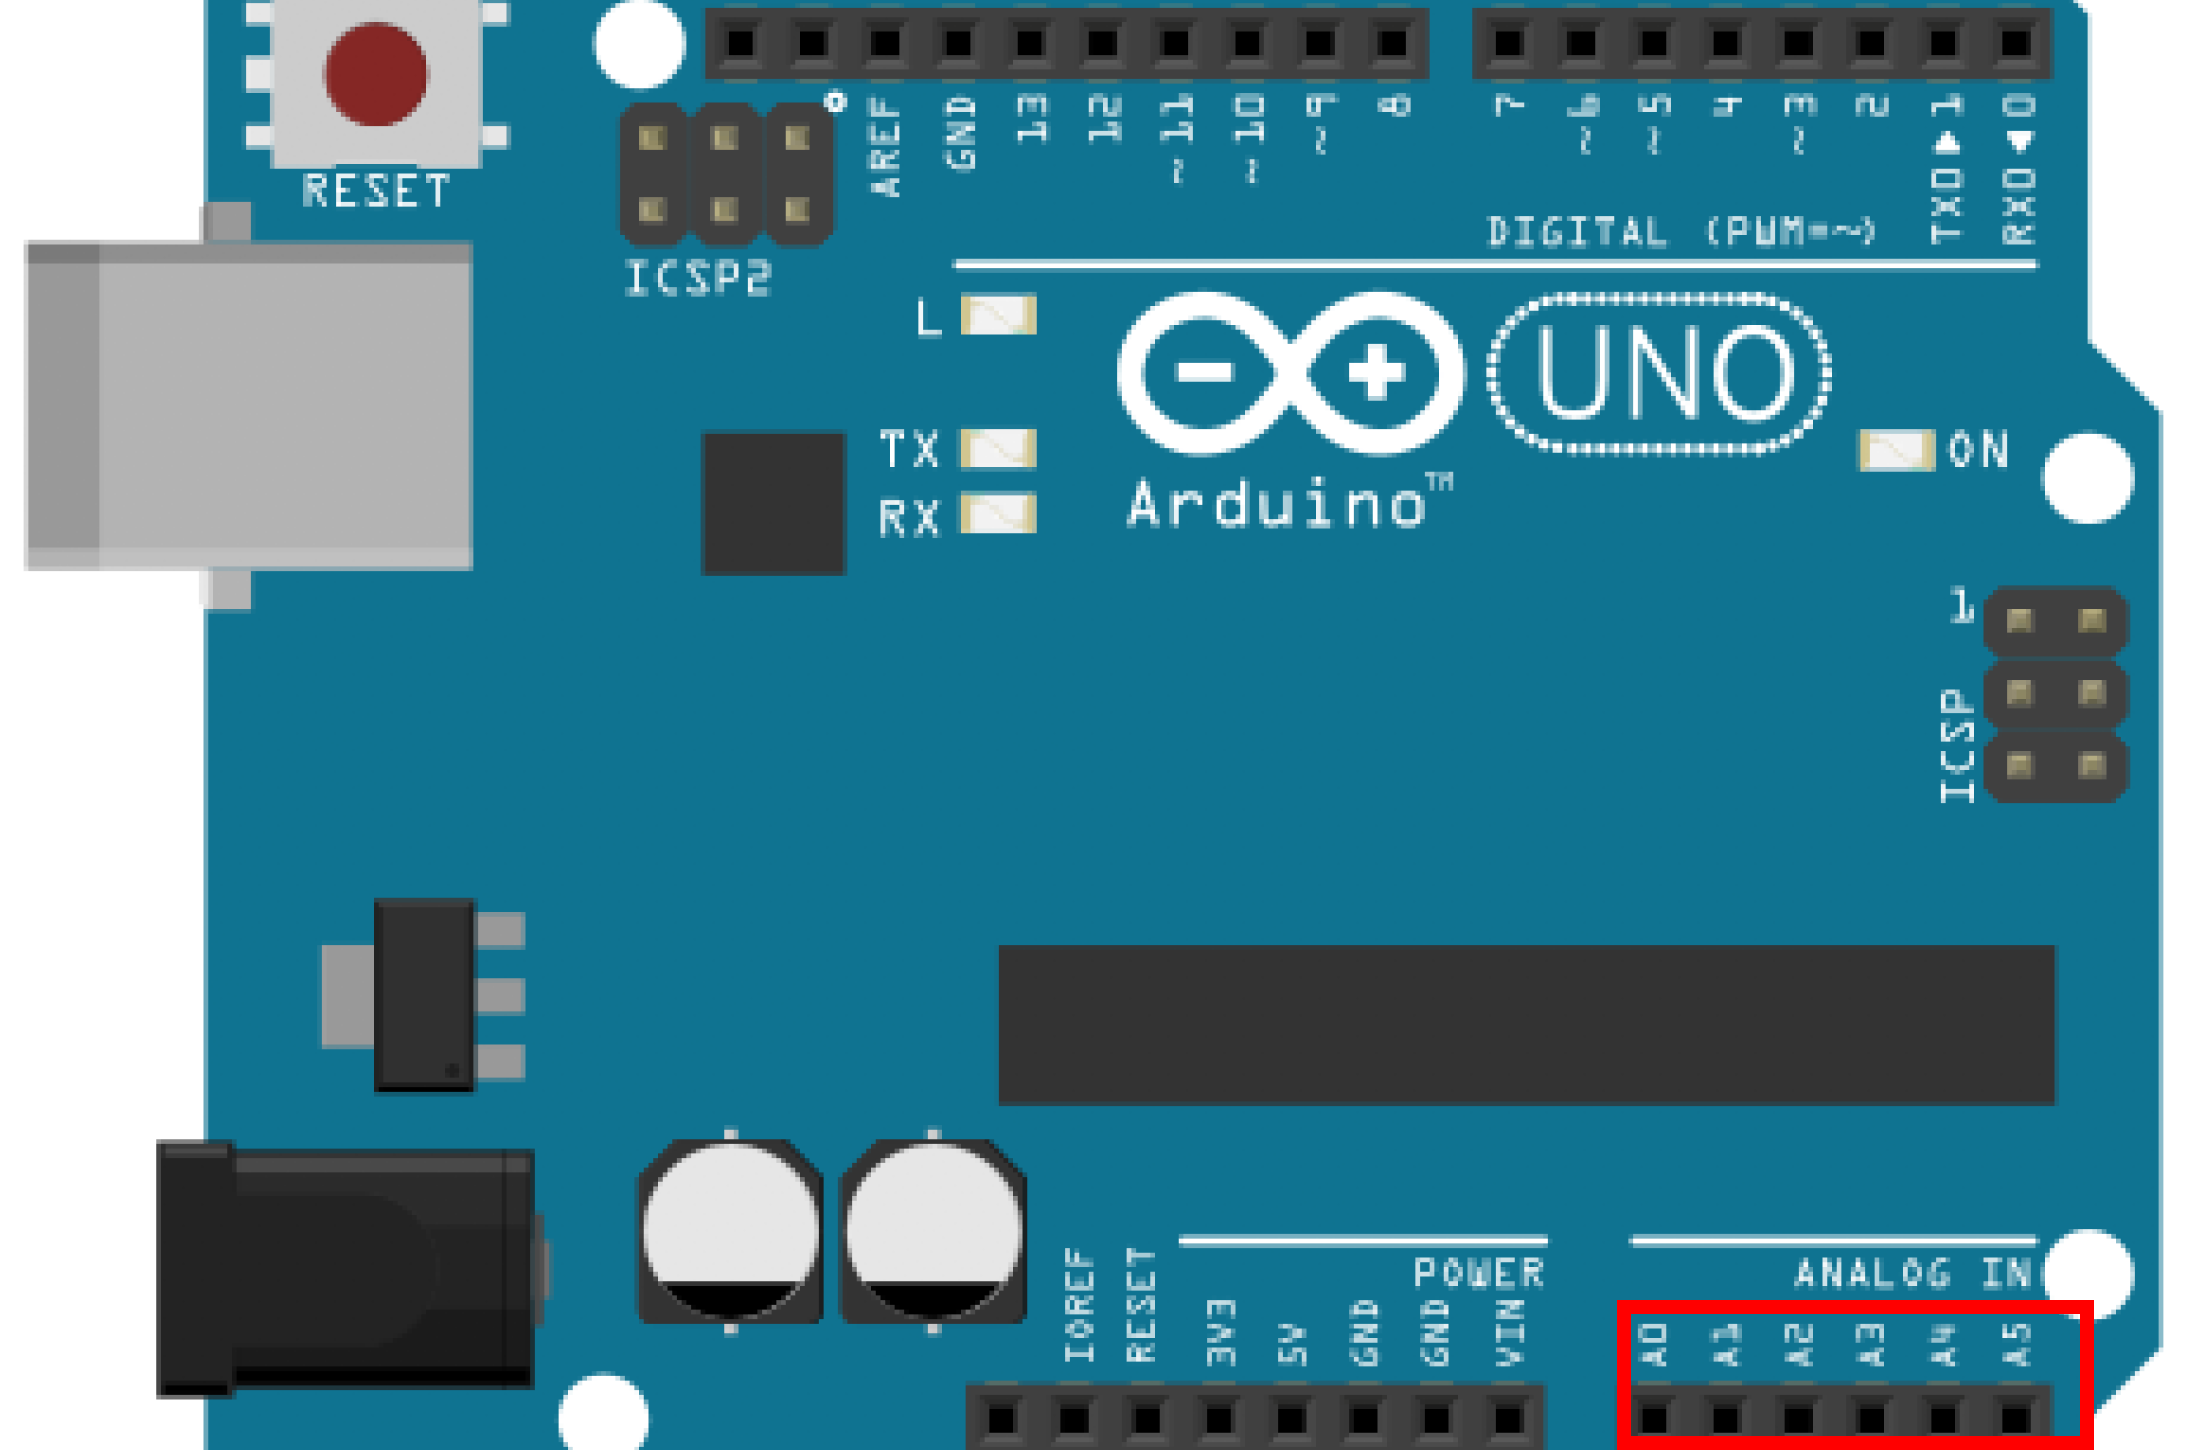
\includegraphics[width=0.8\linewidth]{P5/img/per1/step 8.png}
			\caption{Step 8}
			\label{fig:Step 8(Step 8)}
		\end{figure}

		\item Hubungkan kabel jumper ke salah satu pin GND Arduino, kemudian hubungkan probe.
		\\penjepit buaya (negatif) Function generator.
		\begin{figure}[H]
			\centering
			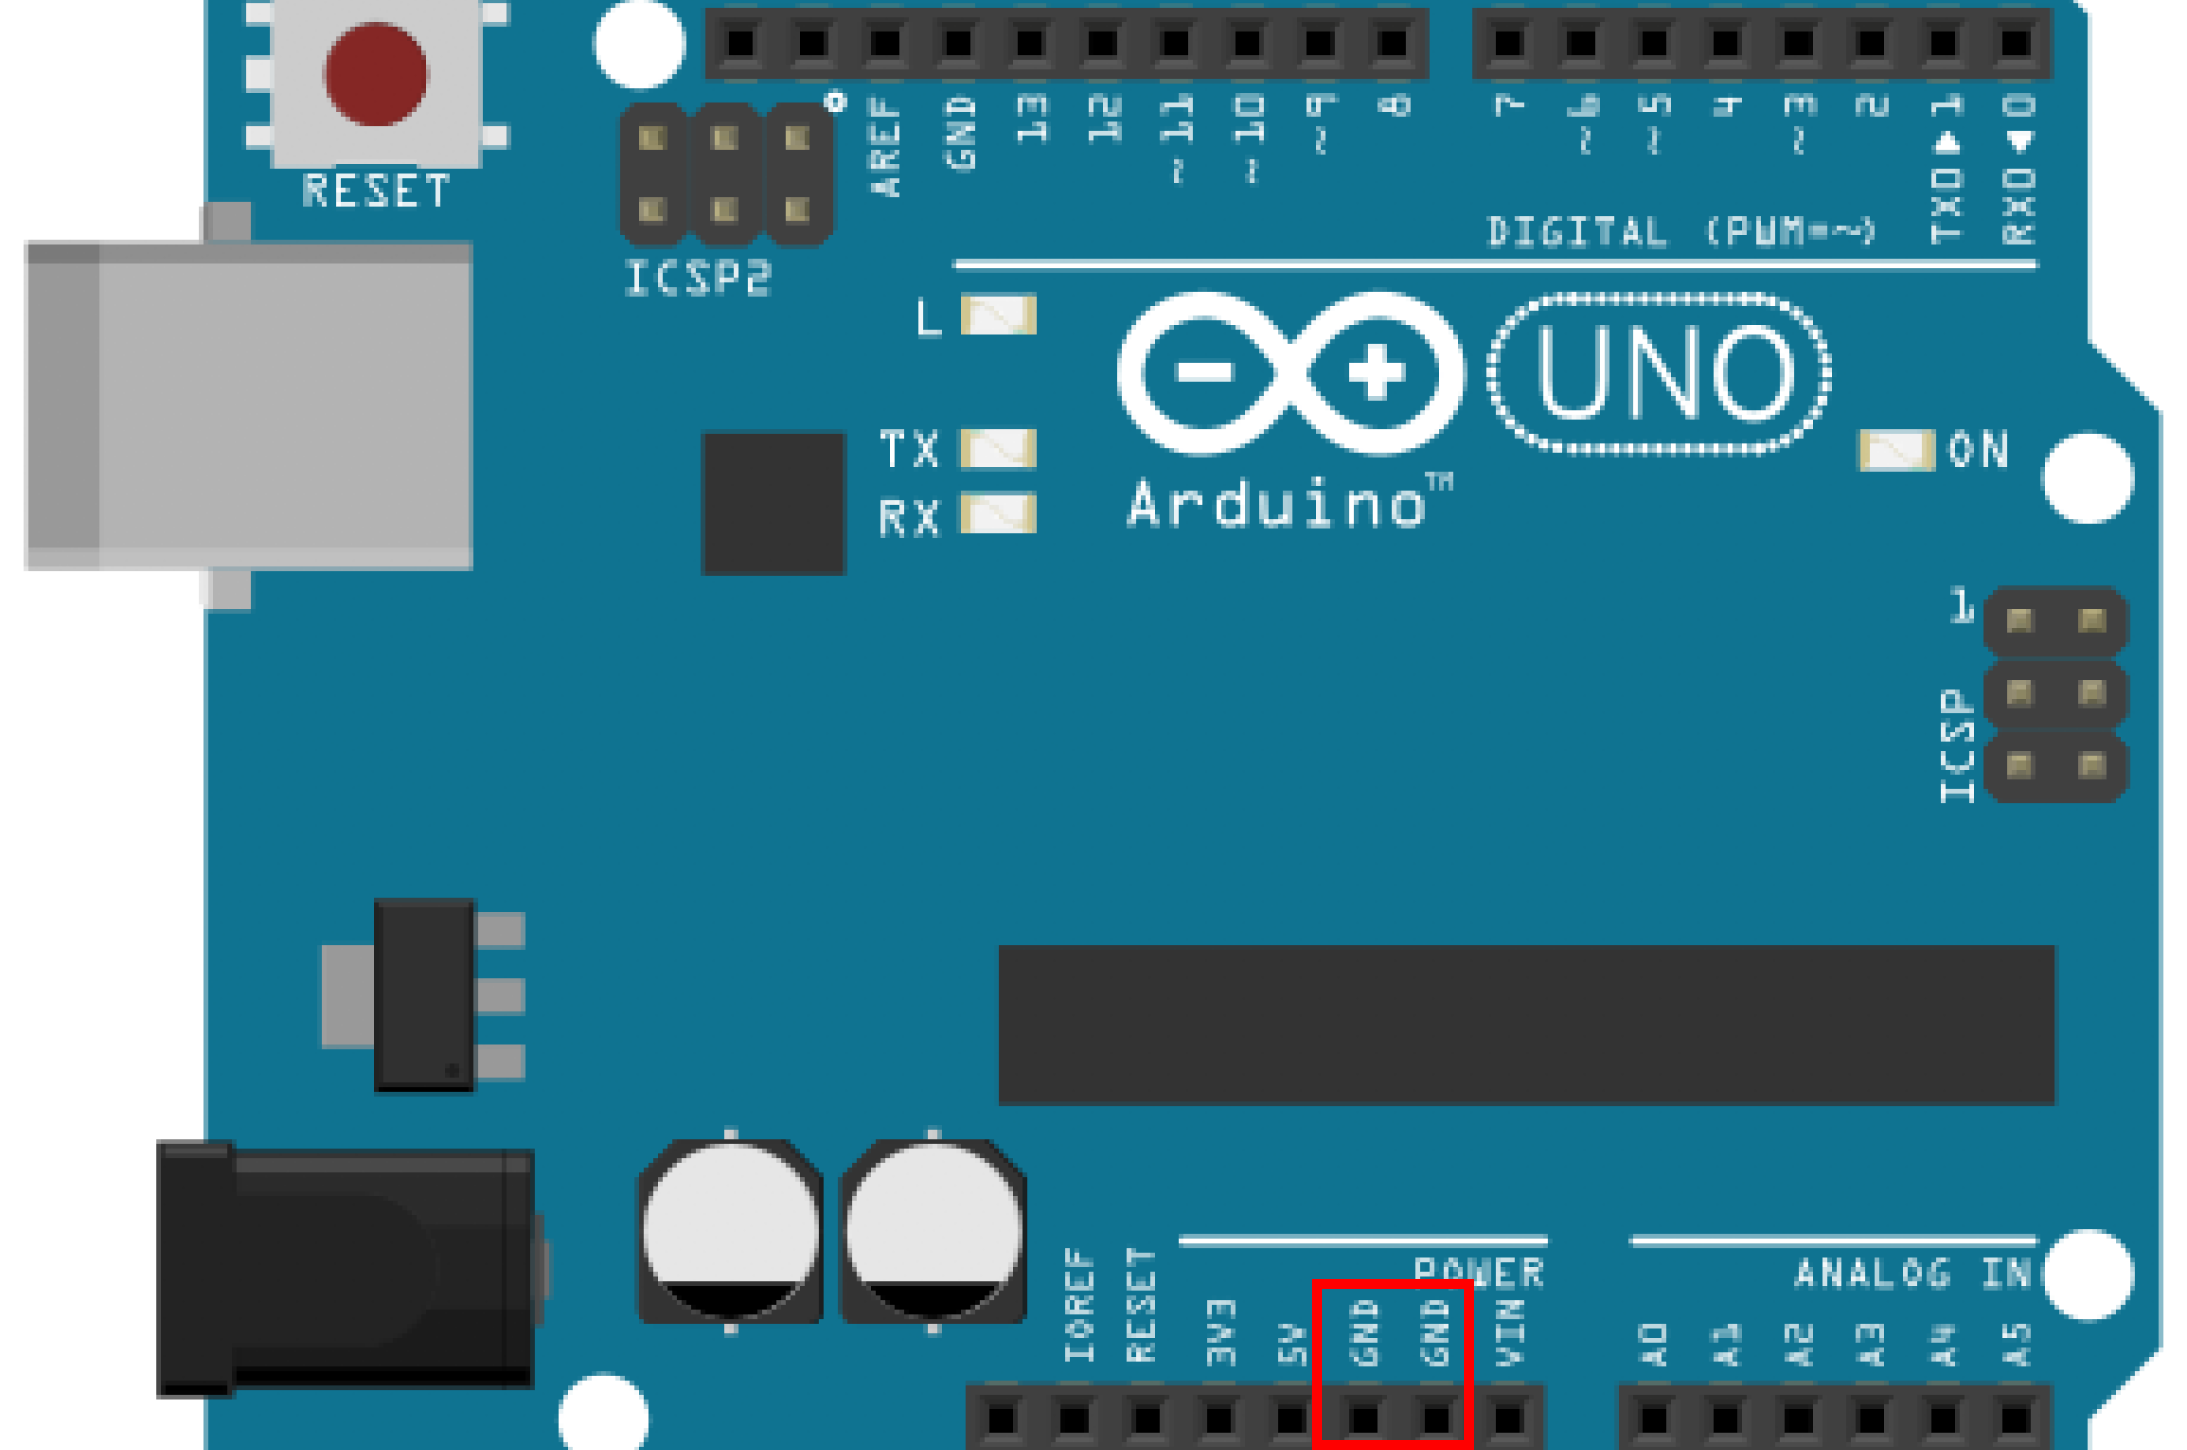
\includegraphics[width=0.8\linewidth]{P5/img/per1/step 9.png}
			\caption{Step 9}
			\label{fig:Step 9(Step 9)}
		\end{figure}

		\item Nyalakan Output 1 pada Function Generator.
		\item Buka Serial plotter di pojok kanan atas pada Arduino IDE.
		\item Buka Serial Monitor di pojok kanan atas pada Arduino IDE.
	\end{enumerate}

\end{center}

%======================PERCOBAAN 2==========================%
\subsection{Percobaan 2}
\begin{center}
	\textbf{Konfigurasi Osiloskop}
	\begin{enumerate}
		\item Hubungkan kabel power ke osiloskop, lalu tekan tombol power untuk menyalakan Osiloskop. 
		\begin{figure}[H]
			\centering
			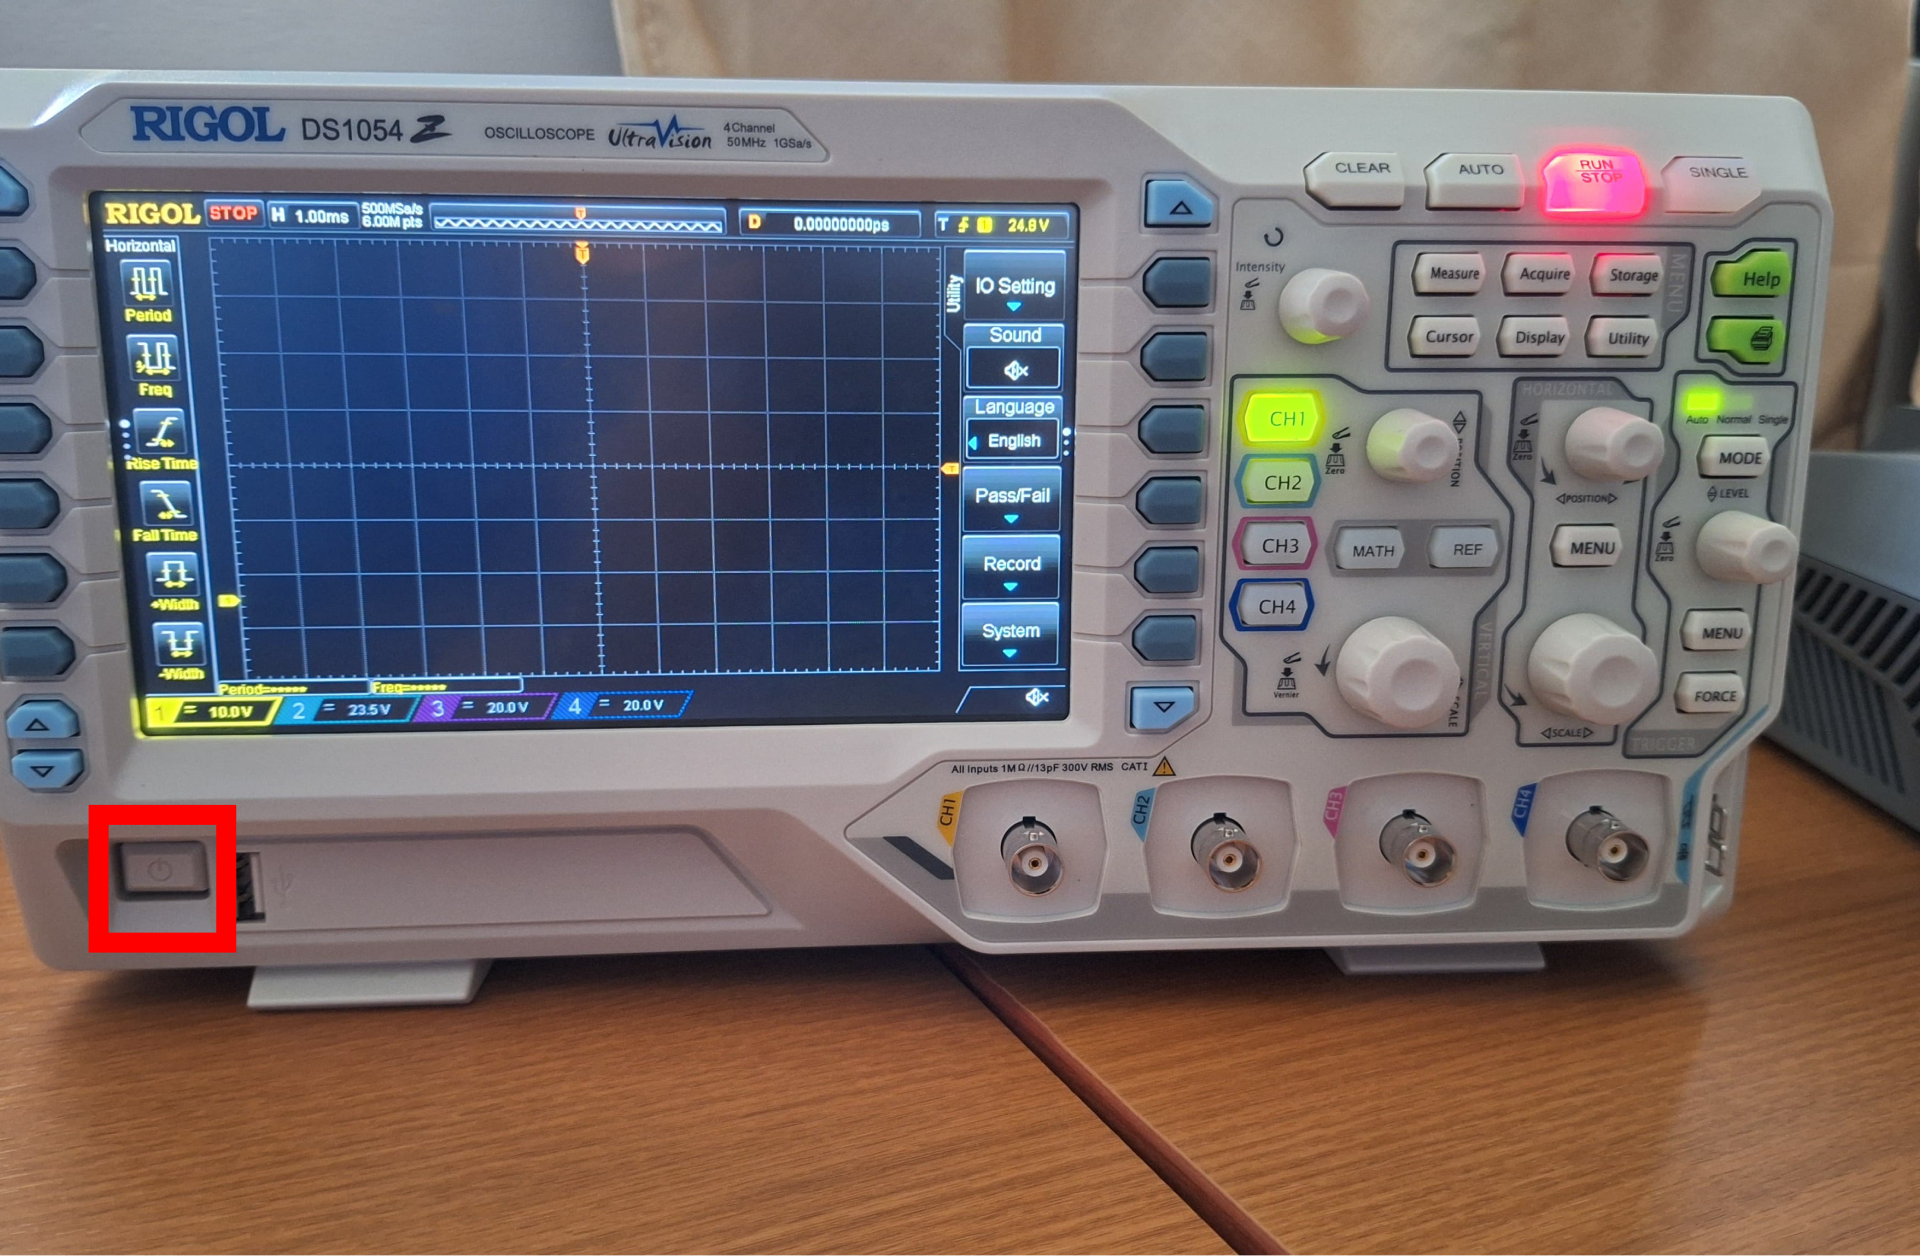
\includegraphics[width=0.9\linewidth]{P5/img/per2/step 1.png}
			\caption{Step 1}
			\label{fig:Step 1(Step 1)}
		\end{figure}

		\item Hubungkan kabel probe pada channel 1. 
		\begin{figure}[H]
			\centering
			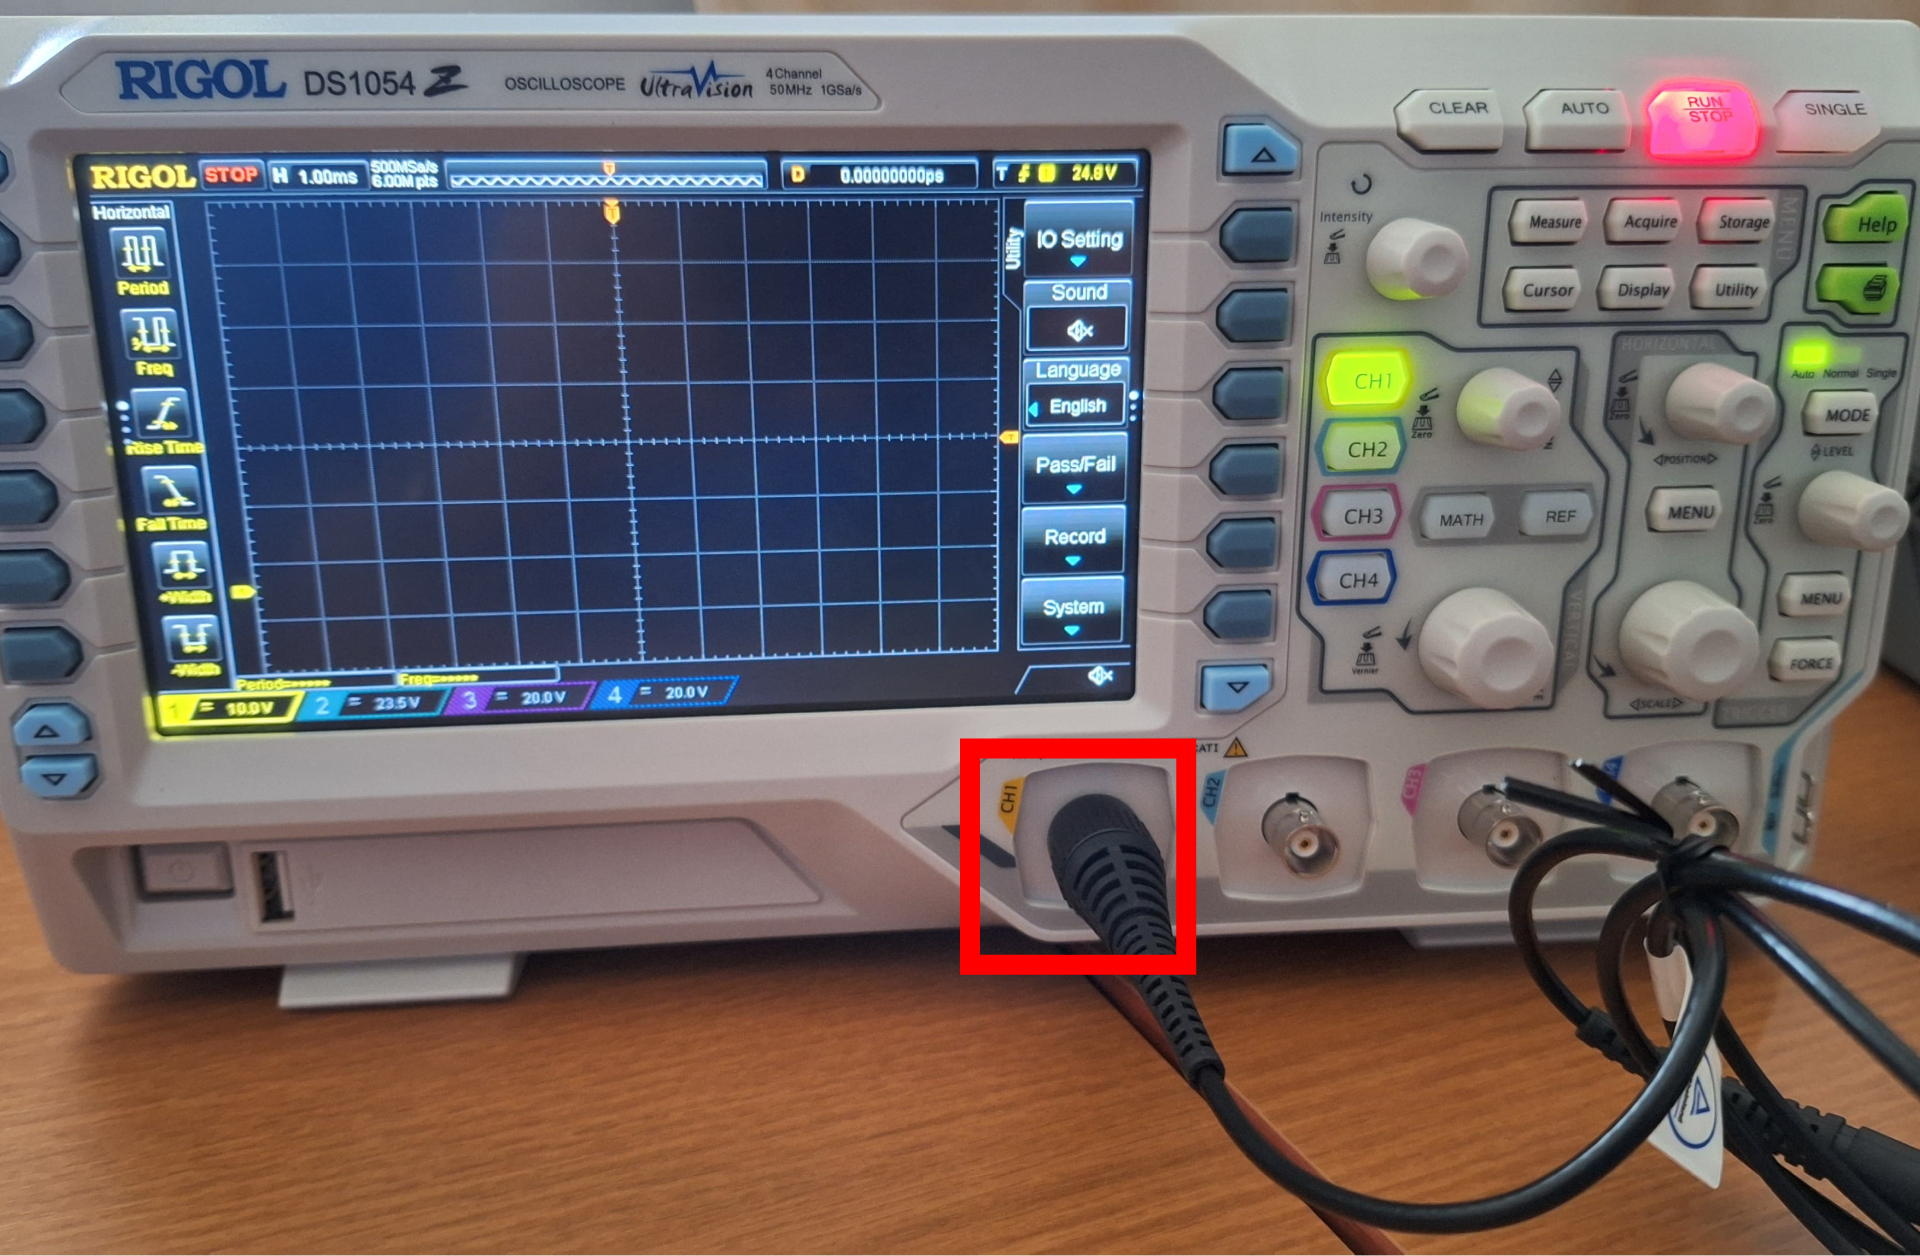
\includegraphics[width=0.8\linewidth]{P5/img/per2/step 2.png}
			\caption{Step 2}
			\label{fig:Step 2(Step 2)}
		\end{figure}

		\item Hubungkan kabel jumper dari salah satu pin Analog Arduino dengan probe pengait (positif) osiloskop dan function generator.
		\item Hubungkan kabel jumper pin GND Arduino dengan probe penjepit buaya (negatif) osiloskop.
		\item Klik AUTO pada Osiloskop.
		\item Bandingkan hasil sinyal yang ditampilkan oleh Serial plotter Arduino dengan Osiloskop.
	\end{enumerate}	
\end{center}

%===========================================================%
\section{Hasil yang didapat}
Memahami perbedaan hasil sinyal digital yang diperoleh oleh Arduino dan Osiloskop.

%===========================================================%
\section{Kesimpulan}
Mengetahui hasil sinyal manakah yang lebih baik dihasilkan dari kedua perangkat \\Arduino dan Osiloskop.
